\documentclass[tikz, usenames, dvipsnames]{standalone}
\usepackage{pgfplots}
\usepgfplotslibrary{groupplots}
\pgfplotsset{height=7cm, compat=1.18}
\usepackage{tikz}
\usepackage{gensymb}
\usepackage{amsmath}
\usepackage[outline]{contour}
\contournumber{64}% default is 16, star form uses 32
\contourlength{.12em}% default is 0.03em
\usetikzlibrary {arrows.meta} 
\usetikzlibrary{decorations.pathreplacing, calligraphy}
\usepgfplotslibrary{fillbetween}

\def\myline{very thick}
% psi = arctan (b sin phi / (a+b cos phi))
\def\psilow{0.89605}

\begin{document}
	
	
	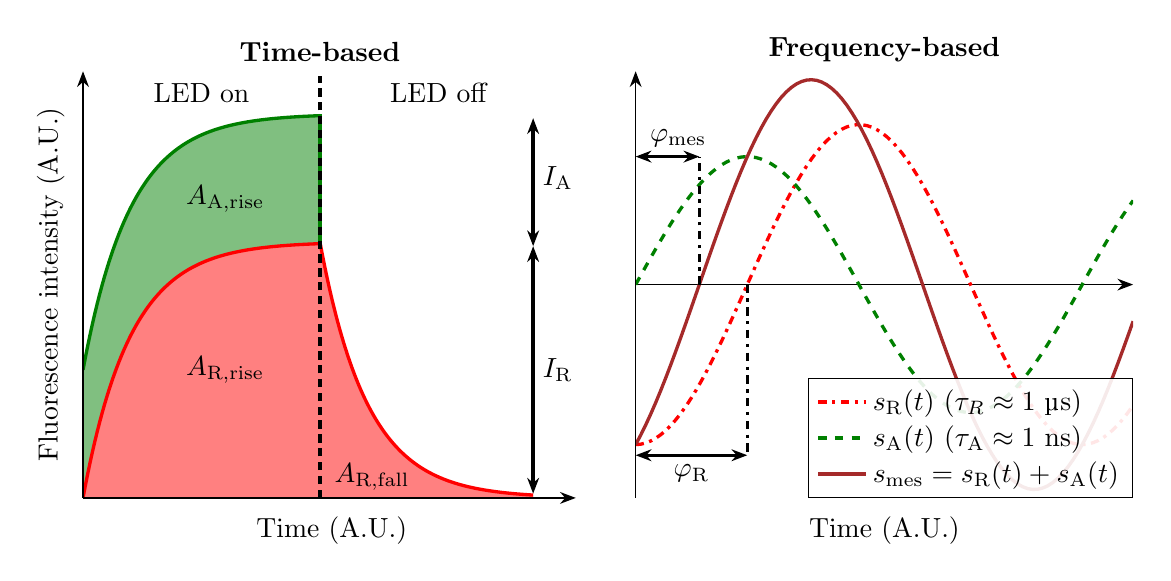
\begin{tikzpicture}	
		%\draw[draw=black] (-1,-1) rectangle ++(14.5cm,7cm);
		\begin{groupplot}[group style={group size=2 by 1, horizontal sep=0.7cm}]
			%
			\nextgroupplot[
			width=7.9cm,
			legend cell align={left},
			tick align=outside,
			tick pos=left,
			xlabel={Time (A.U.)},
			xmin=0, xmax=10.5,
			xtick style={draw=none},
			xticklabels={},
			xlabel style={yshift=8pt},
			ylabel={Fluorescence intensity (A.U.)},
			ylabel style={yshift=-8pt},
			ymin=0, ymax=1,
			ytick style={color=black},
			yticklabels={},
			ytick style={draw=none},
			axis line style={draw=none},
			clip mode=individual,
			domain=0:7,
			samples=100
			]
			
			% Rise
			\addplot[draw=red, no marks, \myline, domain=0:5.01, name path=risephospho] {0.6*(1-exp(-x/1))};
			\addplot[draw=Green, no marks, \myline, domain=0:5, name path=risefluo] {0.6*(1-exp(-x/1)) + 0.3};
			\addplot[draw=none, no marks, \myline, domain=0:5, name path=risex] {0};
			
			% Fall
			\draw[draw=Green, no marks, \myline] (axis cs:5,0.6) -- (axis cs:5,0.9);
			\addplot[draw=red, no marks, \myline, domain=5:9.5, name path=fallphospho] {0.6*exp(-(x-5)/1))};
			\addplot[draw=none, no marks, \myline, domain=5:9.5, name path=fallx] {0};
			
			\addplot[Green!50] fill between[of=risephospho and risefluo];
			\addplot[red!50] fill between[of=risephospho and risex];
			\addplot[red!50] fill between[of=fallphospho and fallx];
			
			% xaxis
			\draw[-{Stealth[length=2mm]}, semithick] (0, 0) -- (10.4, 0); 
			
			% yaxis
			\draw[-{Stealth[length=2mm]}, semithick] (0,0) -- (0,1);
			
			% I
			\draw[{Stealth[length=2mm]}-{Stealth[length=2mm]}, \myline] (9.5, 0.01) -- (9.5, 0.59);
			\node[anchor=west] at (axis cs:9.5, 0.3) {$I_\text{R}$};
			\draw[{Stealth[length=2mm]}-{Stealth[length=2mm]}, \myline] (9.5, 0.59) -- (9.5, 0.89);
			\node[anchor=west] at (axis cs:9.5, 0.75) {$I_\text{A}$};
			
			% A
			\node[anchor=center] at (axis cs:3, 0.7) {$A_\text{A,rise}$};
			\node[anchor=center] at (axis cs:3, 0.3) {$A_\text{R,rise}$};
			\node[anchor=center] at (axis cs:6.1, 0.05) {$A_\text{R,fall}$};
			
			% LED ON/OFF			
			\node[anchor=center] at (axis cs:2.5, 0.95) {LED on};
			\node[anchor=center] at (axis cs:7.5, 0.95) {LED off};
			\draw[draw=black, no marks, \myline, densely dashed] (axis cs:5,0) -- (axis cs:5,0.99);
			
			
			% Title			
			\node[anchor=south] at (axis cs:5, 1) {\textbf{Time-based}};
			
			%%%%%%%%%%%%%%%%%%%%%%%%%%%%%%%%%
			%%%%%%%%%%%%%%%%%%%%%%%%%%%%%%%%%
			
			\nextgroupplot[
			width=7.9cm,
			legend cell align={left},
			tick align=outside,
			tick pos=left,
			xlabel={Time (A.U.)},
			xmin=0, xmax=7,
			xtick style={draw=none},
			xticklabels={},
			xlabel style={yshift=8pt},
			ylabel style={draw=none},
			ymin=-1, ymax=1,
			ytick style={color=black},
			yticklabels={},
			ytick style={draw=none},
			axis line style={draw=none},
			clip mode=individual,
			domain=0:7,
			samples=100,
			legend style={
				fill opacity=.9,
				draw opacity=1,
				text opacity=1,
				at={(axis cs:7,-1.)},
				anchor=south east,
				draw=black
			},
			]
			% xaxis
			\draw[-{Stealth[length=2mm]}, semithick] (0, 0) -- (7, 0); 
			
			\addplot[red, no marks, \myline, , dashdotted] {0.75*sin(180/pi*x - 90)};
			\addlegendentry{$s_\text{R}(t)$ ($\tau_R \approx 1$~\textmu{}s)}
			\addplot[Green, no marks, \myline, dashed] {0.6*sin(180/pi*x)};
			\addlegendentry{$s_\text{A}(t)$ ($\tau_\text{A}\approx 1$~ns)}
			\addplot[Brown, no marks, \myline] {0.6*sin(180/pi*x) + 0.75*sin(180/pi*x - 90)};
			\addlegendentry{$s_\text{mes} = s_\text{R}(t) + s_\text{A}(t)$}
			
			% phi R stuff
			\draw[black, \myline, dashdotted] (pi/2, 0) -- (pi/2, -0.8);
			\draw[{Stealth[length=2mm]}-{Stealth[length=2mm]}, \myline] (0, -0.8) -- (pi/2, -0.8);
			\node[anchor=north] at (axis cs:pi/4, -0.8) {$\varphi_\text{R}$};
			
			% phi mes stuff
			\draw[black, \myline, dashdotted] (\psilow, 0) -- (\psilow, 0.6);
			\draw[{Stealth[length=2mm]}-{Stealth[length=2mm]}, \myline] (0, 0.6) -- (\psilow, 0.6);
			\node[anchor=south] at (axis cs:\psilow/2+0.15, 0.6) {$\varphi_\text{mes}$};
			
			% yaxis
			\draw[-{Stealth[length=2mm]}, semithick] (0,-1) -- (0,1);
			
			% Title
			\node[anchor=south] at (axis cs:3.5, 1) {\textbf{Frequency-based}};
		\end{groupplot}
	\end{tikzpicture}
\end{document}